\let\negmedspace\undefined
\let\negthickspace\undefined
\documentclass[journal]{IEEEtran}
\usepackage[a5paper, margin=10mm, onecolumn]{geometry}
%\usepackage{lmodern} % Ensure lmodern is loaded for pdflatex
\usepackage{tfrupee} % Include tfrupee package

\setlength{\headheight}{1cm} % Set the height of the header box
\setlength{\headsep}{0mm}     % Set the distance between the header box and the top of the text

\usepackage{gvv-book}
\usepackage{gvv}
\usepackage{cite}
\usepackage{amsmath,amssymb,amsfonts,amsthm}
\usepackage{algorithmic}
\usepackage{graphicx}
\usepackage{textcomp}
\usepackage{xcolor}
\usepackage{txfonts}
\usepackage{listings}
\usepackage{enumitem}
\usepackage{mathtools}
\usepackage{gensymb}
\usepackage{comment}
\usepackage[breaklinks=true]{hyperref}
\usepackage{tkz-euclide} 
\usepackage{listings}
% \usepackage{gvv}                                        
\def\inputGnumericTable{}                                 
\usepackage[latin1]{inputenc}                                
\usepackage{color}                                            
\usepackage{array}                                            
\usepackage{longtable}                                       
\usepackage{calc}                                             
\usepackage{multirow}                                         
\usepackage{hhline}                                           
\usepackage{ifthen}                                           
\usepackage{lscape}
\usepackage{circuitikz}
\tikzstyle{block} = [rectangle, draw, fill=blue!20, 
    text width=4em, text centered, rounded corners, minimum height=3em]
\tikzstyle{sum} = [draw, fill=blue!10, circle, minimum size=1cm, node distance=1.5cm]
\tikzstyle{input} = [coordinate]
\tikzstyle{output} = [coordinate]


\begin{document}

\bibliographystyle{IEEEtran}
\vspace{3cm}

\title{4.10.15}
\author{EE25BTECH11013 - Bhargav}
\maketitle
{\let\newpage\relax\maketitle}

\renewcommand{\thefigure}{\theenumi}
\renewcommand{\thetable}{\theenumi}
\setlength{\intextsep}{10pt} % Space between text and floats

\numberwithin{equation}{enumi}
\numberwithin{figure}{enumi}
\renewcommand{\thetable}{\theenumi}

\textbf{Question}:\\
Show that the lines
\begin{align}
\frac{x-1}{2} = \frac{y-2}{3} = \frac{z-3}{4}
\end{align}
and
\begin{align}
\frac{x-4}{5} = \frac{y-1}{2} = z
\end{align}
intersect. Also, find their point of intersection.\\

\solution \\

The vector equations of the given lines are
\begin{align}
\vec{r}_1 &= \myvec{1\\2\\3} + \lambda \myvec{2\\3\\4}, \\
\vec{r}_2 &= \myvec{4\\1\\0} + \mu \myvec{5\\2\\1}.
\end{align}

At the point of intersection,
\begin{align}
\vec{r}_1 = \vec{r}_2.
\end{align}

Thus,
\begin{align}
\myvec{1\\2\\3} + \lambda \myvec{2\\3\\4} &= \myvec{4\\1\\0} + \mu \myvec{5\\2\\1}.
\end{align}

This can be written as a matrix equation:
\begin{align}
\myvec{2 & -5 \\ 3 & -2 \\ 4 & -1}\myvec{\lambda \\ \mu} = \myvec{3 \\ -1 \\ -3}.
\end{align}

The corresponding augmented matrix is
\begin{align}
\augvec{2}{1}{2 & -5 &3 \\ 3 & -2 &  -1 \\ 4 & -1 & -3} \xleftrightarrow[R_2 \leftarrow R_2 - \frac{3}{2}R_1]{R_3 \leftarrow R_3 - 2R_1} \augvec{2}{1}{2 & -5 & 3 \\ 0 & \frac{11}{2} & \frac{-11}{2} \\ 0 & 9 & -9} \xleftrightarrow[R_3 \leftarrow 11R_3 - 9R_2]{R_2 \leftarrow 2R_2} \augvec{2}{1}{2 & -5 & 3 \\ 0 & 11 & -11 \\ 0 & 0 & 0}
\end{align}

\begin{align}
\implies \myvec{\lambda \\ \mu} = \myvec{-1 \\ -1}
\end{align}


Substituting into $\vec{r}_1$:
\begin{align}
\vec{r}_1 = \myvec{1\\2\\3} + (-1)\myvec{2\\3\\4} = \myvec{-1\\-1\\-1}.
\end{align}

$\therefore$ the lines intersect at the point
\begin{align}
\myvec{-1\\-1\\-1}
\end{align}

\begin{figure}[h!]
    \centering
    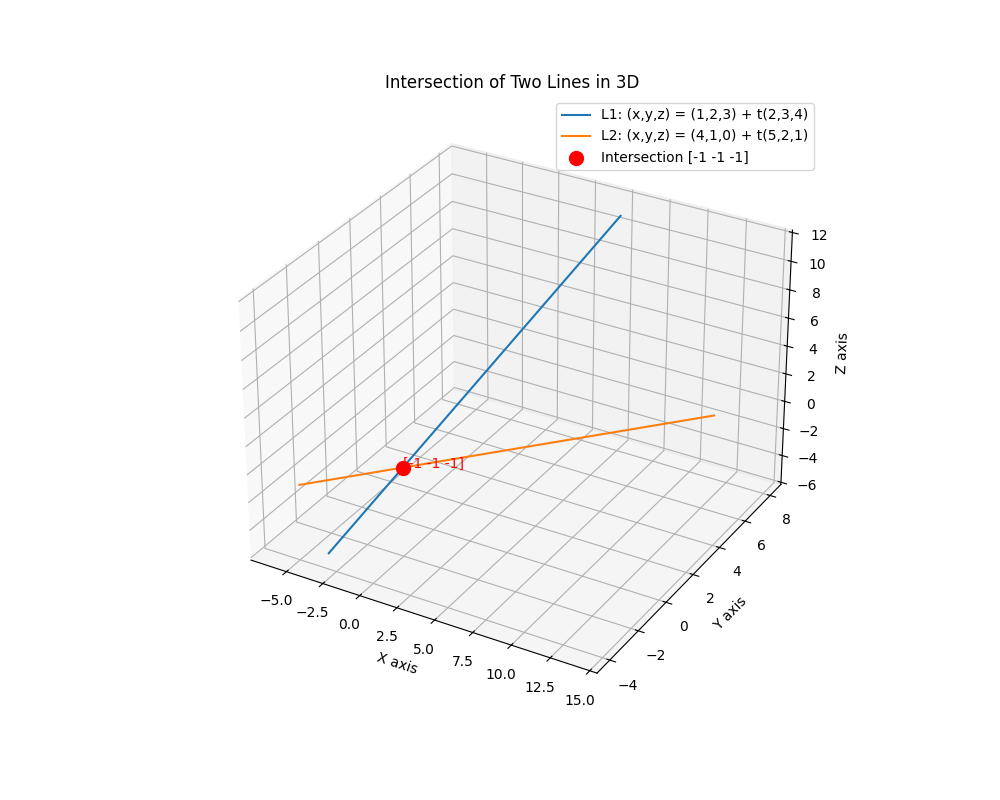
\includegraphics[height=0.5\textheight, keepaspectratio]{figs/Figure_1.png}
    \label{figure_1}
\end{figure}


\end{document}

